% DYSLEXIA SWITCH
\newif\ifdys
		
				% ENABLE or DISABLE font change
				% use XeLaTeX if true
				\dystrue
				\dysfalse


\ifdys

\documentclass[a4paper, 14pt]{extarticle}
\usepackage{amsmath,amsfonts,amsthm,amssymb,mathtools}

\tracinglostchars=3 % Report an error if a font does not have a symbol.
\usepackage{fontspec}
\usepackage{unicode-math}
\defaultfontfeatures{ Ligatures=TeX,
                      Scale=MatchUppercase }

\setmainfont{OpenDyslexic}[Scale=1.0]
\setmathfont{Fira Math} % Or maybe try KPMath-Sans?
\setmathfont{OpenDyslexic Italic}[range=it/{Latin,latin}]
\setmathfont{OpenDyslexic}[range=up/{Latin,latin,num}]

\else

\documentclass[a4paper, 12pt]{extarticle}

\usepackage[utf8x]{inputenc}
\usepackage{lmodern,textcomp}
\usepackage{amsmath,amsfonts,amsthm,amssymb,mathtools}

\fi


\usepackage[french]{babel}
\usepackage[
a4paper,
margin=2cm,
nomarginpar,% We don't want any margin paragraphs
]{geometry}
\usepackage{icomma}

\usepackage{fancyhdr}
\usepackage{array}
\usepackage{hyperref}

\usepackage{multicol, enumerate}
\newcolumntype{P}[1]{>{\centering\arraybackslash}p{#1}}


\usepackage{stackengine}
\newcommand\xrowht[2][0]{\addstackgap[.5\dimexpr#2\relax]{\vphantom{#1}}}

% theorems

\theoremstyle{plain}
\newtheorem{theorem}{Th\'eor\`eme}
\newtheorem*{sol}{Solution}
\theoremstyle{definition}
\newtheorem{ex}{Exercice}

% corps
\newcommand{\C}{\mathbb{C}}
\newcommand{\R}{\mathbb{R}}
\newcommand{\Rnn}{\mathbb{R}^{2n}}
\newcommand{\Z}{\mathbb{Z}}
\newcommand{\N}{\mathbb{N}}
\newcommand{\Q}{\mathbb{Q}}

% domain
\newcommand{\D}{\mathbb{D}}


% date
\usepackage{advdate}
\AdvanceDate[1]


% plots
\usepackage{pgfplots}

% table line break
\usepackage{makecell}


% SOLUTION SWITCH
\newif\ifsolutions
				\solutionstrue
				%\solutionsfalse

\ifsolutions
	\newcommand{\exe}[2]{
		\begin{ex} #1  \end{ex}
		\begin{sol} #2 \end{sol}
	}
\else
	\newcommand{\exe}[2]{
		\begin{ex} #1  \end{ex}
	}
	
\fi

\begin{document}
\pagestyle{fancy}
\fancyhead[L]{Seconde 13}
\fancyhead[C]{\textbf{Statistiques 2 \ifsolutions -- Solutions  \fi}}
\fancyhead[R]{\today}

\exe{\footnote{\href{https://www.insee.fr/fr/statistiques/4277635}{https://www.insee.fr/fr/statistiques/4277635}} \par
	En 2019, 753 000 bébés sont nés en France, soit 6 000  naissances de moins qu’en 2018 ($– 0,7\%$). Le nombre de naissances baisse chaque année depuis cinq ans, mais à un rythme qui ralentit au fil des années. Alors que la baisse était de 2,4 \% en 2015, elle est passée à 1,9 \% en 2016 puis 1,8 \% en 2017, 1,4 \% en 2018 et enfin 0,7 \% en 2019. En France métropolitaine, le nombre de naissances s’établit à 714 000. Il reste plus élevé que le point bas de 1994 (711 000).
	
	\begin{center}
	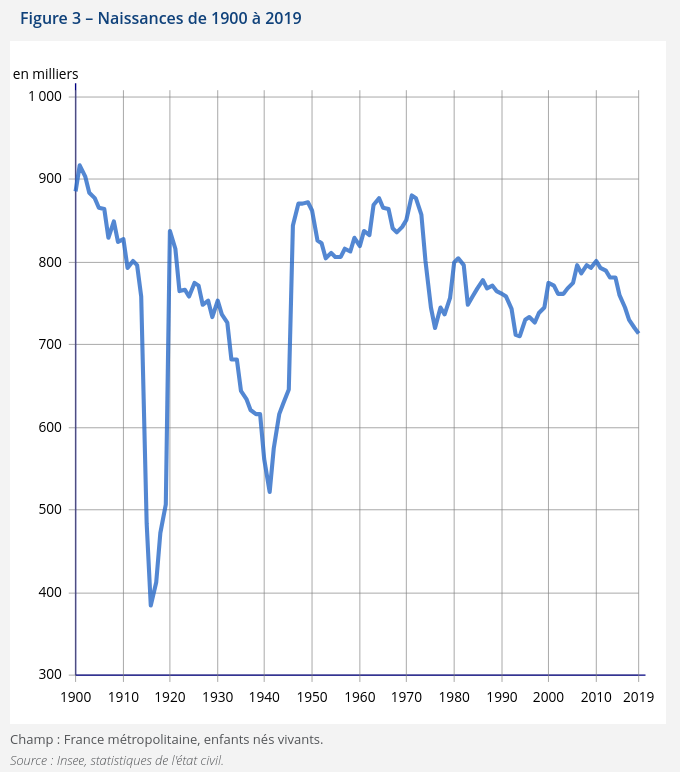
\includegraphics[scale=0.55]{fig.png}
	\end{center}
	
	\begin{enumerate}
		\item Calculer, à l'aide du texte, le nombre de bébés nés en France en $2018, 2017, 2016, 2015$, et $2014$.
		Comparer avec la figure 3.
		
		\item Calculer l'évolution relative du nombre de bébés nés en France métropolitaine entre $1994$ et $2019$.
		
		\item Calculer l'évolution relative du nombre de bébés nés en France métropolitaine entre $1971$ et $1976$.
		
		\item Donner approximativement le nombre de bébés nés en France métropolitaine en $1916$ et en $1941$. Expliquer les pics de natalité.
		
		\item Calculer et comparer les évolutions relatives de natalité d'après-guerre : entre $1916$ et $1920$ contre $1941$ et $1947$.
	\end{enumerate}
}{

	\begin{enumerate}
		\item Du texte on déduit les évolutions suivantes.
		
		\begin{tabular}{|c|c|c|c|c|c|}\hline
			Année & 2019 & 2018 & 2017 & 2016 & 2015 \\ \hline
			Évolution & -0,7\% & -1,4\% & -1,8\% & -1,9\% & -2,4\% \\ \hline
		\end{tabular}
		
		L'année $2018$ est en fait déjà donné par le texte à $753+6 = 759$ milliers de naissances.
		
		Pour l'année $2017$, on utilise l'évolution de $-1,4\%$.
		
		On calcule donc que, pour retourner en arrière, l'évolution réciproque de $+1,4\%$ correspond à un coefficient multiplicatif de 
			\[ 1-\dfrac{1,4}{100} = 0,983. \]
		L'évolution réciproque est alors donnée par $\dfrac{1}{0,986}$, qui multipliée à $759$ donne environ $770$.
		
		\begin{tabular}{|c|c|c|c|c|c|c|}\hline
			Année & 2019 & 2018 & 2017 & 2016 & 2015 & 2014 \\ \hline
			\makecell{Nombre de  naissances \\ (approximativement, en milliers)} & 753 & 759 & 770 & 784 & 799 & 819 \\ \hline
		\end{tabular}
		
		On remarque que les valeurs obtenues sont en dessous de celles du graphique qui n'indique $800$ mille naissances qu'en $2010$.
		C'est parce que celui-ci ne concerne que la France métropolitaine.
		
		\item 
		Le texte nous donne deux valeurs : 711 mille en 1994, et 714 mille en 2019.
		La proportion est donnée par 
			\[ \dfrac{714}{711} \approx 1,004. \]
		Comme $1,004 - 1 = 0,004 = 0,4\%$, le nombre de bébés nés en France métropolitaine a augmenté de 0,4\% entre 1994 et 2019.
		
		\item
		On lit graphiquement (et donc approximativement) les valeurs pour obtenir une proportion d'environ
			\[ \approx \dfrac{725}{880} \approx 0,82. \]
		Il s'agit d'une diminution d'environ $1-0,82 = 18\%$.
		
		\item 
		La figure nous indique environ $390$ mille naissances en 1916 et $520$ mille naissances en 1941.
		Ces valeurs sont prises en pendant la Première et la Seconde Guerre mondiale (et au moins $9$ mois après leur début !).
		
		\item Entre $1916$ et $1920$ on calcule un proportion d'environ
			\[ \dfrac{840}{390} \approx 2,15, \]
		qui correspond à une évolution de $2,15-1 = 115\%$.
		
		Entre $1941$ et $1947$ on calcule une proportion d'environ
			\[ \dfrac{880}{520} \approx 1,69, \]
		qui correspond à une évolution de $1,69 - 1 = 69\%$.
		
		Les natalités après la Seconde Guerre mondiale sont \underline{relativement} moins importante comparé à la Première Guerre mondiale. 
		Cependant, les valeurs hautes de natalités persistent dans le temps jusqu'en $1974$ — c'est le baby-boom.
		
	\end{enumerate}
}

\ifsolutions
\else
\newpage
\fi

\exe{\footnote{\href{https://www.insee.fr/fr/statistiques/7750004}{https://www.insee.fr/fr/statistiques/7750004}}\par
	%Au 1er janvier 2024, la France compte 68,4 millions d’habitants (figure 1) : 66,1 millions résident en France métropolitaine et 2,2 millions dans les cinq départements d’outre-mer. La population augmente de 0,3 \% sur un an, comme en 2022. Le rythme de croissance annuel était plus élevé auparavant : +0,4 \% pour les années 2019 à 2021 et +0,5 \% en 2017 et en 2018.
	
	En 2023, le \emph{solde naturel}, différence entre les nombres de naissances et de décès enregistrés sur l’année, est de +47 000, son plus bas niveau depuis la fin de la Seconde Guerre mondiale. En baisse régulière depuis 2007, le solde naturel a chuté en 2020 sous l’effet d’une baisse des naissances, mais surtout d’une forte hausse des décès due à la pandémie de Covid-19. Depuis, il est resté à un niveau bas. Il s’était légèrement redressé en 2021 sous l’effet d’un rebond des naissances, mais il a diminué en 2022, les décès restant à un niveau élevé. Il baisse de nouveau en 2023, les naissances diminuant plus fortement que les décès (figure 2a).
	
	\begin{center}
	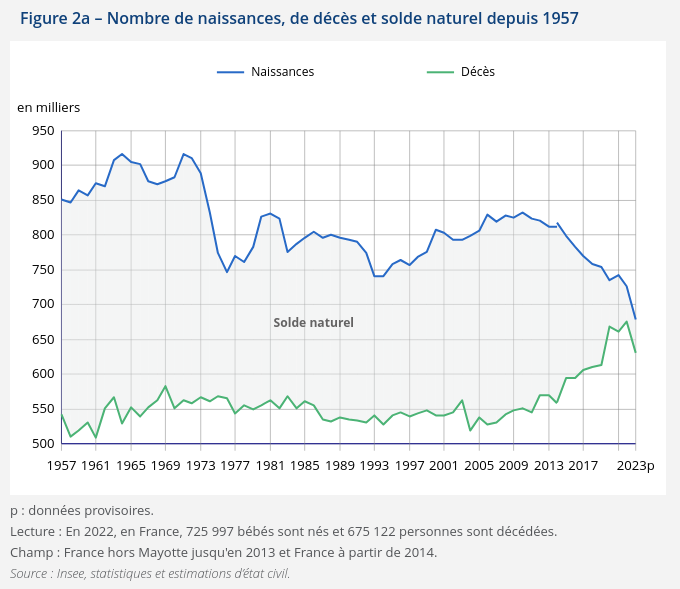
\includegraphics[scale=0.75]{fig2.png}
	\end{center}
	
	
	\begin{enumerate}
		%\item Calculer approximativement la population française en début d'années $2023, 2022, \dots, 2017$.
		
		\item Approximer les évolutions relatives des naissances et des décès entre $2022$ et $2023$. Comparer.
		
		\item Calculer approximativement l'évolution relative du solde naturel entre les années $1971$ et $1976$.
		
		\item Estimer l'évolution relative du solde naturel entre $2020$ et $2021$, puis entre $2021$ et $2022$.
		En déduire, par le calcul, l'évolution relative entre $2020$ et $2022$.

	\end{enumerate}
}{
	\begin{enumerate}
		\item 
		On lit graphiquement (et donc approximativement) les valeurs suivantes.
		
		\begin{tabular}{|c|c|c|}\hline
			Année & 2022 & 2023 \\ \hline
			Naissances (milliers) & 730 & 680 \\ \hline
			Décès (milliers) & 675 & 630 \\ \hline
		\end{tabular}

		On en conclut les évolutions suivantes.
		\begin{enumerate}[i)]
			\item $1-\dfrac{680}{730} \approx 7\%$ de diminution des naissances.
			\item $1- \dfrac{630}{675} \approx 6,6\%$ de diminution des décès.
		\end{enumerate}
		
		Ainsi les naissances et les décès diminuent tous deux, mais les naissances diminuent relativement plus en $2022$ à $2023$.
		
		\item 
		En approximant le solde naturel en $1971$ et $1976$, on obtient environ $ \approx 920 - 560 = 360$ mille, et $775 - 570 = 205$ mille.
		
		La diminution est donc donnée par $1-\dfrac{205}{306} \approx 43\%$.
		
		\item 
		Les soldes naturels en $2020, 2021,$ et $2022$ sont approximativement égaux à $65$, $85$, $55$.
		
		De $2020$ à $2021$, il y a donc eu une augmentation de $\dfrac{85}{65}- 1 \approx 30\%$.
		De $2021$ à $2022$, il y a eu une diminution de $1-\dfrac{55}{85} \approx 35\%$.
		
		Le coefficient multiplicatif pour passer du solde en $2020$ au solde en $2022$ est donc environ $1,3 \cdot 0,65 \approx 0,88$, qui correspond à une diminution de $12\%$.
		On vérifie avec les valeurs connues : $1-\dfrac{55}{65} \approx 15\%$.
		
	\end{enumerate}
		
	En conclusion, en approximant deux évolutions locales puis en les multipliant pour trouver une évolution globale, on additionne les erreurs commises et notre résultat n'est pas assez précis.
	On trouve environ $12\%$, au lieu des $15\%$ par calcul direct.
	
	Plus généralement, l'approximation répétée est dangereuse en calcul numérique. 
	C'est d'ailleurs un champ d'étude important en algorithmique, où tout est approximé, faute de précision infinie.
}
\end{document}
